\documentclass[border=15pt]{standalone}
\usepackage{tikz}
\usepackage{amsmath}
\usepackage{amssymb}
\usetikzlibrary{shadows, positioning, shapes.geometric, calc, arrows.meta}

% Macros based on your definitions
\newcommand{\vect}[1]{\boldsymbol{#1}}
\newcommand{\F}{\mathbb{F}}
\newcommand{\code}{\mathcal{C}}

% Consistent color palette
\definecolor{accent}{HTML}{1F4E79}
\definecolor{softaccent}{HTML}{EAF2F8}
\definecolor{softgray}{HTML}{F6F7F9}

\begin{document}
	
	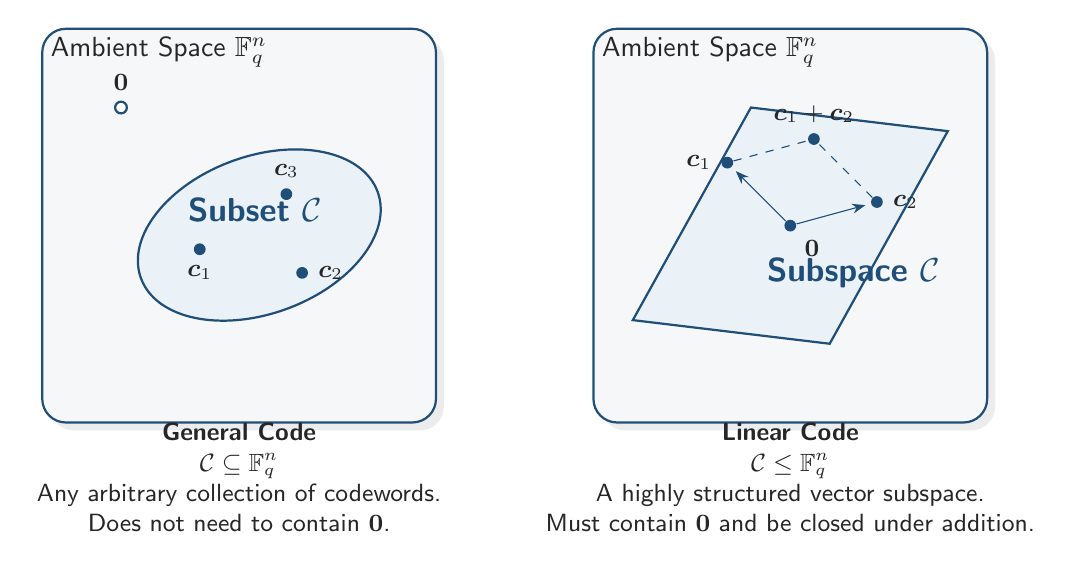
\begin{tikzpicture}[
		>=Stealth,
		ambient/.style={
			draw=accent, thick, fill=softgray, rounded corners=3mm, 
			minimum width=5cm, minimum height=5cm,
			drop shadow={opacity=0.15, shadow xshift=1mm, shadow yshift=-1mm}
		},
		labeltext/.style={font=\sffamily, text=black!85},
		header/.style={font=\bfseries\sffamily\large, text=accent},
		codeword/.style={circle, fill=accent, inner sep=1.5pt}
		]
		
		% ==========================================
		% PANEL 1: General Code (Arbitrary Subset)
		% ==========================================
		
		% Ambient Space
		\node[ambient] (space1) at (0,0) {};
		\node[anchor=north west, labeltext, font=\sffamily] at (space1.north west) {Ambient Space $\F_q^n$};
		
		% Arbitrary Subset (Blob)
		\draw[draw=accent, thick, fill=softaccent, rotate around={20:(0,0)}] 
		(0.2, -0.2) ellipse (1.6cm and 1cm);
		\node[header] at (0.2, 0.2) {Subset $\code$};
		
		% Codewords inside the subset
		\node[codeword, label={[labeltext, font=\small]below:$\vect{c}_1$}] at (-0.5, -0.3) {};
		\node[codeword, label={[labeltext, font=\small]right:$\vect{c}_2$}] at (0.8, -0.6) {};
		\node[codeword, label={[labeltext, font=\small]above:$\vect{c}_3$}] at (0.6, 0.4) {};
		
		% The zero vector is explicitly OUTSIDE the code to show it's not required
		\node[circle, draw=accent, thick, inner sep=1.5pt, fill=white, label={[labeltext, font=\small]above:$\vect{0}$}] at (-1.5, 1.5) {};
		
		% Caption
		\node[labeltext, align=center, font=\sffamily\small] at (0, -3.2) {
			\textbf{General Code}\\
			$\code \subseteq \F_q^n$\\
			Any arbitrary collection of codewords.\\
			Does not need to contain $\vect{0}$.
		};
		
		
		% ==========================================
		% PANEL 2: Linear Code (Vector Subspace)
		% ==========================================
		
		% Ambient Space
		\node[ambient] (space2) at (7,0) {};
		\node[anchor=north west, labeltext, font=\sffamily] at (space2.north west) {Ambient Space $\F_q^n$};
		
		% Subspace (A plane passing through the origin)
		\draw[draw=accent, thick, fill=softaccent] 
		(5.0, -1.2) -- (6.5, 1.5) -- (9.0, 1.2) -- (7.5, -1.5) -- cycle;
		\node[header] at (7.8, -0.6) {Subspace $\code$};
		
		% The origin (MUST be in a linear code)
		\node[codeword, label={[labeltext, font=\small]below right:$\vect{0}$}] (zero) at (7,0) {};
		
		% Codewords demonstrating linear combinations
		\node[codeword, label={[labeltext, font=\small]left:$\vect{c}_1$}] (c1) at (6.2, 0.8) {};
		\node[codeword, label={[labeltext, font=\small]right:$\vect{c}_2$}] (c2) at (8.1, 0.3) {};
		
		% Vector addition (c1 + c2)
		\node[codeword, label={[labeltext, font=\small]above:$\vect{c}_1+\vect{c}_2$}] (c3) at (7.3, 1.1) {};
		
		% Dashed lines showing the parallelogram of vector addition
		\draw[dashed, accent, thin] (c1) -- (c3);
		\draw[dashed, accent, thin] (c2) -- (c3);
		\draw[->, accent, thin, shorten >=2pt] (zero) -- (c1);
		\draw[->, accent, thin, shorten >=2pt] (zero) -- (c2);
		
		% Caption
		\node[labeltext, align=center, font=\sffamily\small] at (7, -3.2) {
			\textbf{Linear Code}\\
			$\code \leq \F_q^n$\\
			A highly structured vector subspace.\\
			Must contain $\vect{0}$ and be closed under addition.
		};
		
	\end{tikzpicture}
	
\end{document}